% Synthetic seismic sections from Mandyoc scenarios: methods.
% Section to be \input in the manuscript (natbib, amsmath, graphicx, booktabs, siunitx).
% Implementation: seismic_section_parallel.py / seismic_section.py of post_processing.

\section{Synthetic seismic sections}
\label{sec:seismic}

To compare the numerical scenarios with seismic observations of rifted margins
\citep[e.g.][]{Gillard2015, Gillard2016a, Gillard2016b, Gillard2019, Chenin2023}, we converted
the outputs of the thermo-mechanical models into synthetic seismic reflection sections. The
numerical scenarios were simulated with the finite element code Mandyoc
\citep{Sacek2017, Sacek2022, Silva2022, Silva2023}, which provides, at each time step, the
distribution of the lithologies, the temperature and the accumulated strain. However, these
fields are computed on a mesh with elements of the order of 1~km, while the seismic image
depends on structures with dimensions of tens of meters, comparable to the seismic wavelength.
Therefore, most of the steps described below are used to bridge this gap in a physically
motivated way, without changing the geometry of the margin obtained by the numerical model.

The workflow is divided in three main stages (Fig.~\ref{fig:seismic_flowchart}): (1) the
construction of a high-resolution model of density and P-wave velocity ($V_P$) from the
Mandyoc outputs; (2) the calculation of a convolutional section for the whole margin; and
(3) the simulation of the wave propagation and the migration of the synthetic data in a
selected window of the margin.

\begin{figure}[ht]
  \centering
  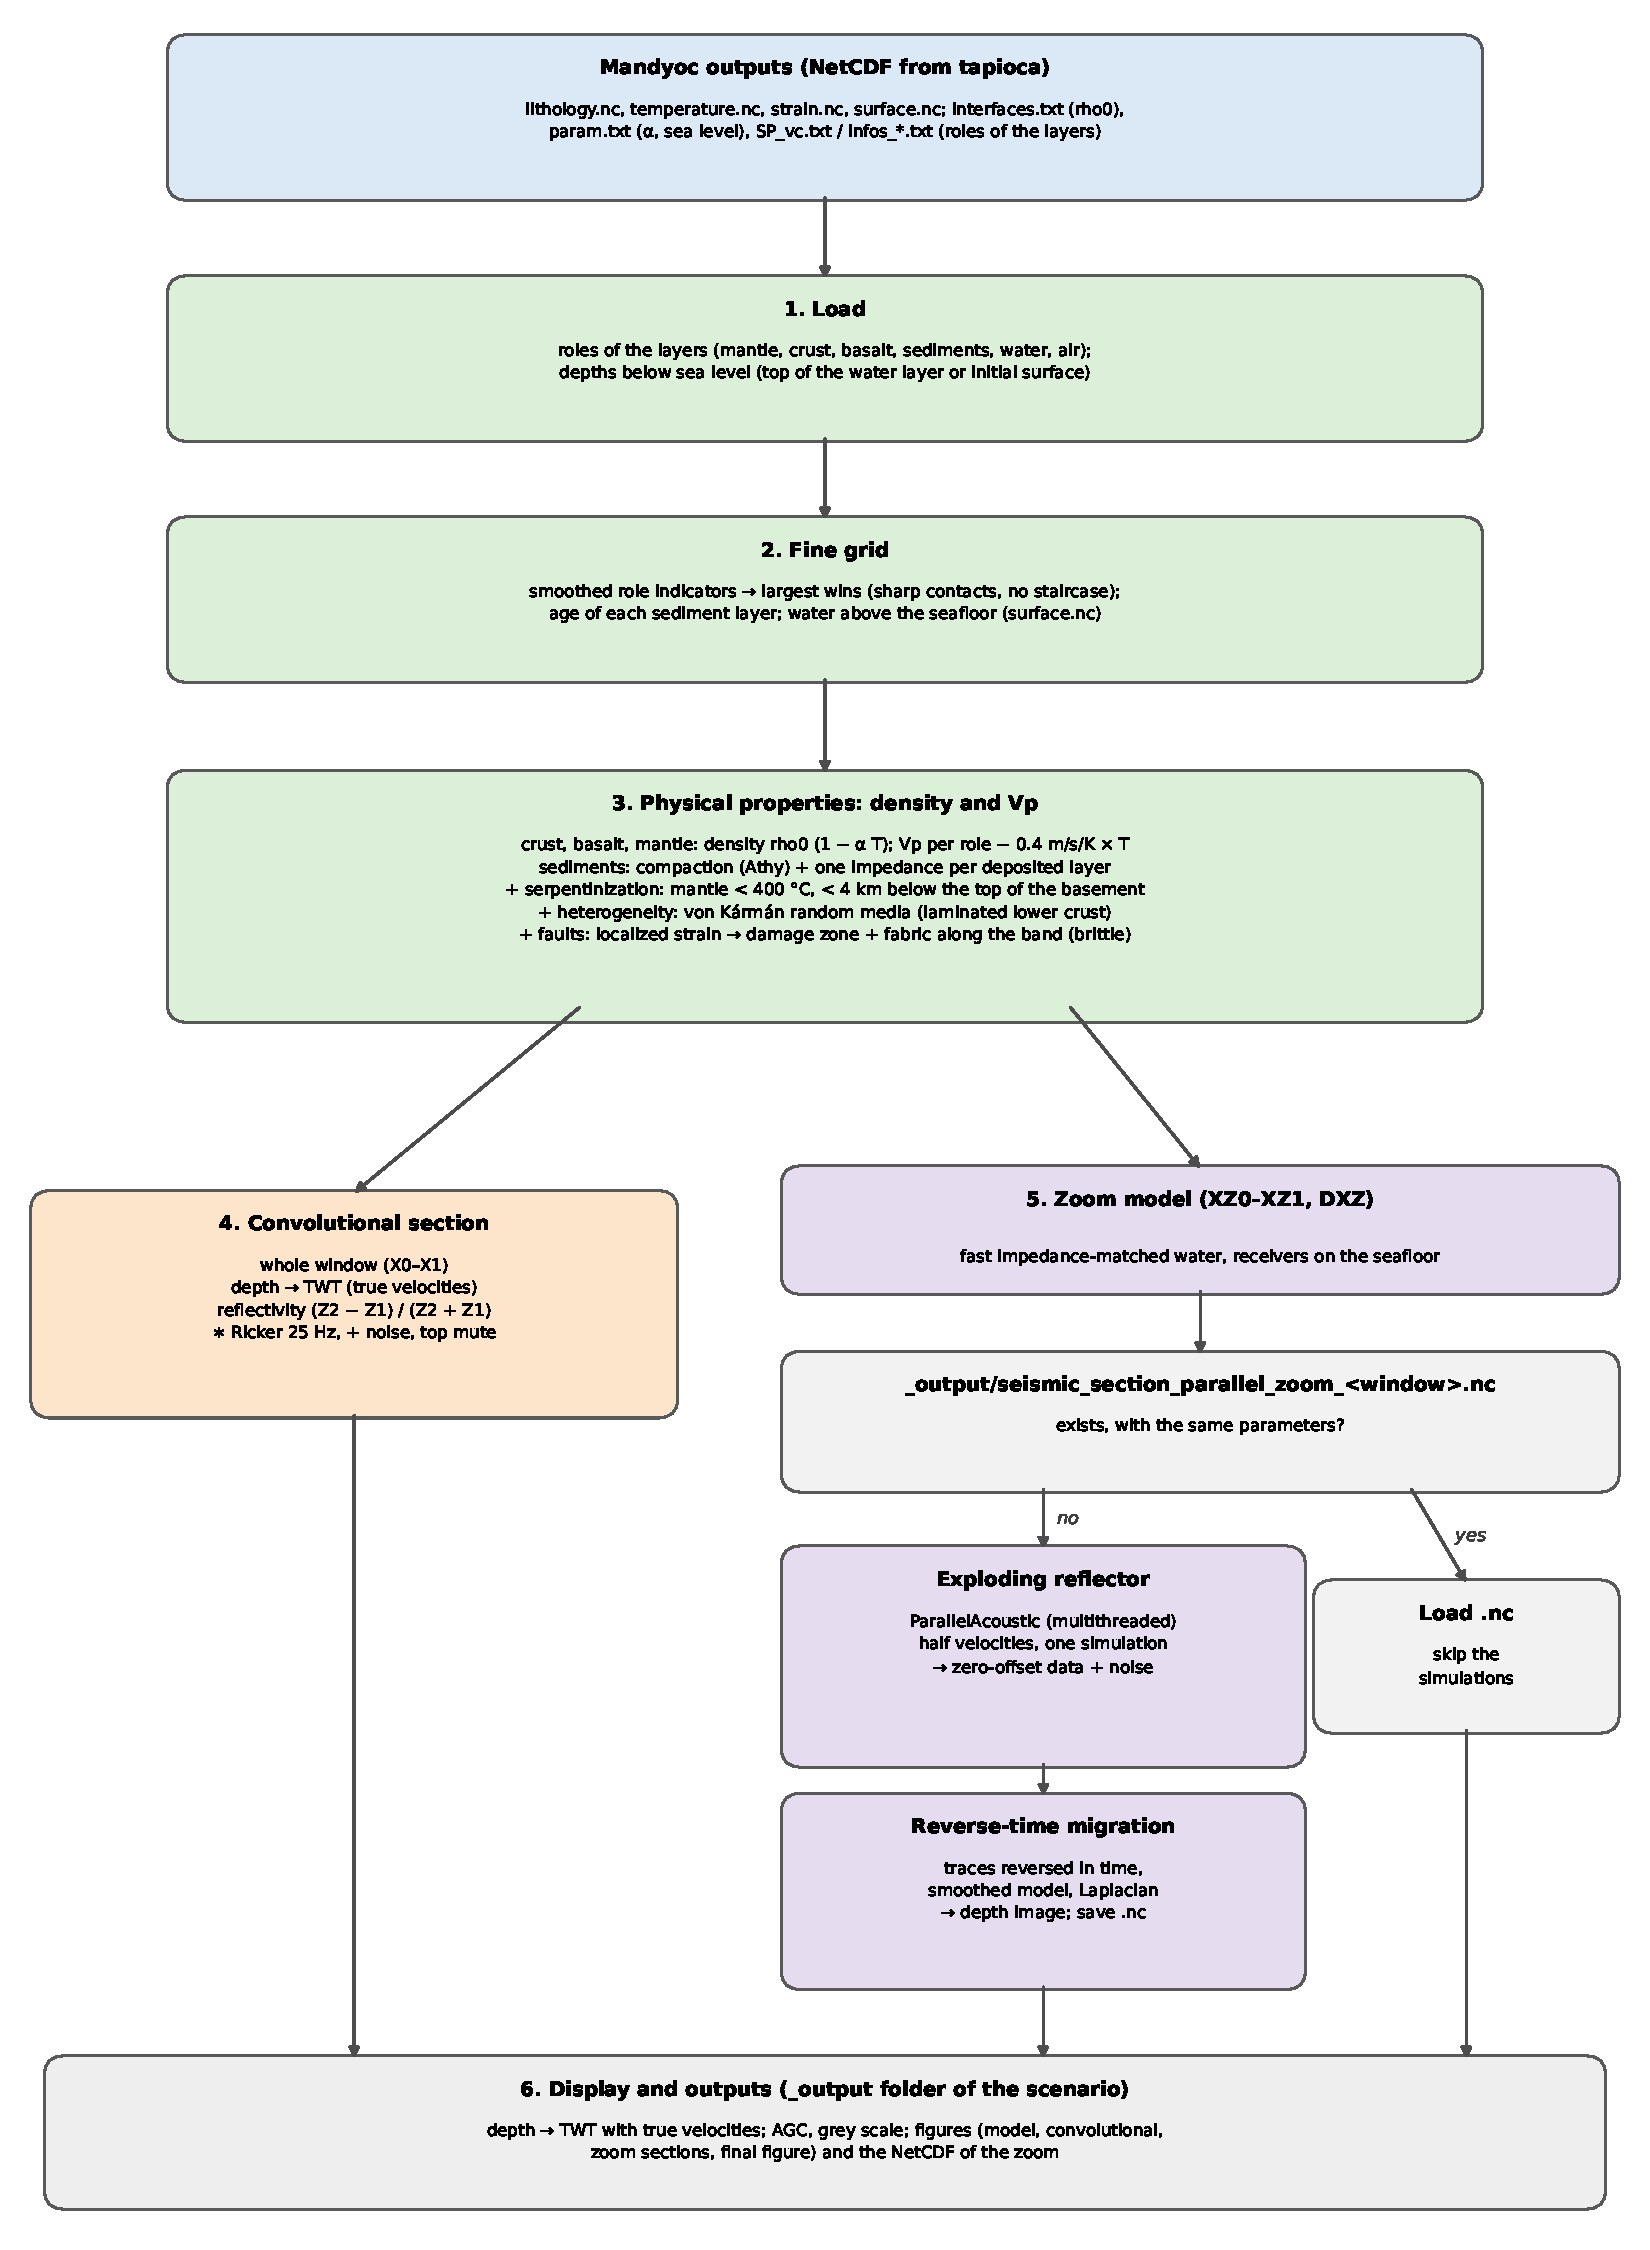
\includegraphics[width=0.75\textwidth]{seismic_flowchart.pdf}
  \caption{Workflow adopted to obtain the synthetic seismic sections from the outputs of
  the Mandyoc scenarios.}
  \label{fig:seismic_flowchart}
\end{figure}

\subsection{Physical properties of the model}
\label{sec:seismic_properties}

\paragraph{Lithology on the fine grid.}
For a selected time step, the lithology, temperature and accumulated strain of the numerical
scenario were interpolated onto a regular grid with spacing $\Delta x = 25$~m, in depth below
sea level. Each Mandyoc layer was assigned to a lithological unit (asthenosphere, lithospheric
mantle, lower crust, upper crust, basalt, sediments, water or air) according to its name or,
when it is not available, its reference density. The layers with density between 2750 and
3200~kg/m$^3$ located above the upper crust were assumed to be basalt, corresponding to the
magma extracted during the simulation. Instead of interpolating the lithology directly, we
smoothed the indicator function of each unit (1 inside and 0 outside of the unit) with a
Gaussian filter with standard deviation of 300~m, and each grid point received the unit with
the largest smoothed value. This procedure keeps the contacts between the units sharp, which
is necessary to produce reflections, but removes the staircase geometry of the numerical mesh,
which would otherwise produce artificial diffractions. The sea level was defined as the top of
the water layer, when the scenario has one, or as the sea level adopted in the Mandyoc
scenario, and all the space between the seafloor and the sea level was filled with water.

\paragraph{Crystalline rocks.}
The density of the crust, basalt and mantle was calculated with the same thermal expansion
adopted in the numerical scenarios:
\begin{equation}
  \rho = \rho_0 (1 - \alpha T),
  \label{eq:seismic_density}
\end{equation}
where $\rho_0$ is the reference density of each layer at 0~$^\circ$C, $\alpha$ is the
coefficient of thermal expansion and $T$ is the temperature. The P-wave velocity was
calculated as:
\begin{equation}
  V_P = V_{P0} + \frac{\partial V_P}{\partial T}\, T,
  \label{eq:seismic_vp}
\end{equation}
where $V_{P0}$ is the velocity at 0~$^\circ$C of each lithological unit (Table~\ref{tab:seismic}),
based on typical values for the continental crust and upper mantle
\citep{Christensen1995}, and $\partial V_P / \partial T = -0.4$~m\,s$^{-1}$\,K$^{-1}$ is a
typical value of the temperature derivative of the velocity of crustal and mantle rocks
\citep{Christensen1979}. With this correction, the hot asthenosphere beneath the rift is
slower than the cold lithospheric mantle, as observed in wide-angle seismic data.

\paragraph{Sediments.}
In the numerical scenarios, the sediments have a constant density, which is not appropriate to
represent their seismic properties. For sediments, the velocity and density are mainly
controlled by compaction, and the porosity $\phi$ decreases exponentially with the burial
depth $h$ below the seafloor \citep{Athy1930}:
\begin{equation}
  \phi = \phi_0 \exp\left(-\frac{h}{\lambda}\right),
  \label{eq:athy}
\end{equation}
where $\phi_0$ is the porosity at the seafloor and $\lambda$ is the compaction length. The
P-wave velocity was calculated with the Wyllie time-average equation \citep{Wyllie1956}:
\begin{equation}
  \frac{1}{V_P} = \frac{\phi}{V_w} + \frac{1 - \phi}{V_m},
  \label{eq:wyllie}
\end{equation}
where $V_w$ and $V_m$ are the velocities of the water and of the rock matrix, respectively,
and the density is given by $\rho = \phi \rho_w + (1 - \phi) \rho_g$, where $\rho_w$ and
$\rho_g$ are the densities of the water and of the grains. With the values of
Table~\ref{tab:seismic}, $V_P$ increases from $\sim$2.2~km/s at the seafloor to $\sim$4.3~km/s
at 5~km below it. Each sediment layer deposited in the numerical scenario (i.e., each time
interval of the surface processes) received its own surface porosity and matrix velocity,
drawn from normal distributions around the mean values (Table~\ref{tab:seismic}). The
resulting impedance contrasts between the deposited layers produce the stratified
reflections, onlaps and sedimentary wedges observed in seismic sections. Note that these
contrasts are statistical and do not represent specific stratigraphic horizons.

\paragraph{Serpentinization.}
At magma-poor rifted margins, the exhumed mantle is serpentinized near the top of the
basement, and the P-wave velocities increase from $\sim$4.3 km/s at the top of the basement
to $\sim$7.3~km/s a few kilometers below it \citep{Minshull2009, Gillard2019}. Since the
numerical scenarios do not simulate the hydration of the mantle, we prescribed a serpentinized
fraction $s$ for the mantle rocks, assuming that serpentinization requires water from the
surface and low temperatures \citep{Martin1970, Reston2007}:
\begin{equation}
  s = \min\left[1, \max\left(0, 1 - \frac{h_b}{H_s}\right)\right]
      \min\left[1, \max\left(0, \frac{T_s - T}{\Delta T}\right)\right],
  \label{eq:serpentinization}
\end{equation}
where $h_b$ is the depth below the top of the basement (the first crystalline rock below the
sediments), $H_s = 4$~km is the maximum depth of serpentinization below the top of the
basement, $T_s = 400$~$^\circ$C is the maximum temperature of serpentinization and
$\Delta T = 50$~$^\circ$C. The velocity and density of the mantle were then linearly mixed with
those of the serpentinite, $V_P = (1 - s) V_P + s V_{serp}$ and
$\rho = (1 - s) \rho + s \rho_{serp}$, with $V_{serp} = 4.3$~km/s and
$\rho_{serp} = 2550$~kg/m$^3$ \citep{Christensen2004, Carlson2003}.

\paragraph{Small-scale heterogeneity.}
The rocks of the basement are not homogeneous, and their internal reflectivity is responsible
for the texture of the seismic sections. We represented this heterogeneity with von
K\'arm\'an random media, commonly used to describe the small-scale heterogeneity of the crust
in studies of seismic scattering \citep{Frankel1986, Sato2012}. In each lithological unit, the
velocity was perturbed as $V_P \rightarrow V_P (1 + \delta)$, where $\delta$ is a random field
with standard deviation $\varepsilon$ and power spectrum:
\begin{equation}
  P(k_{\parallel}, k_{\perp}) \propto
  \left(1 + k_{\parallel}^2 a_{\parallel}^2 + k_{\perp}^2 a_{\perp}^2\right)^{-(\nu + 1)},
  \label{eq:von_karman}
\end{equation}
where $k_{\parallel}$ and $k_{\perp}$ are the wavenumbers along and across the fabric of the
rock, $a_{\parallel}$ and $a_{\perp}$ are the respective correlation lengths and $\nu = 0.3$
is the Hurst exponent. The density was perturbed accordingly, with
$\delta \ln \rho = 0.25\, \delta \ln V_P$. The perturbations are of a few percent
(Table~\ref{tab:seismic}) and change only the velocities inside each unit, preserving the
geometry of the margin. The lower continental crust is commonly laminated and reflective
\citep{Holliger1992}, so its perturbations are elongated horizontally ($a_{\parallel} = 4$~km,
$a_{\perp} = 150$~m), while the upper crust has weaker and more isotropic perturbations, the
mantle is nearly transparent and the serpentinized mantle is the most heterogeneous unit. In
the sediments, only weak variations along each deposited layer were added.

\paragraph{Fault zones.}
The faults, detachments and shear zones formed during the numerical simulation are recorded
in the accumulated strain field. To keep only the localized deformation, we removed the
regional trend of the accumulated strain $\varepsilon_{acc}$ with a Gaussian high-pass filter:
\begin{equation}
  \varepsilon_{loc} = \max\left[0, \varepsilon_{acc} - G_{\sigma} * \varepsilon_{acc}\right],
  \label{eq:localized_strain}
\end{equation}
where $G_{\sigma}$ is a Gaussian kernel with standard deviation $\sigma = 4$~km, and
$\varepsilon_{loc}$ was normalized by its 99th percentile. Discrete faults are expected only
in the brittle domain, so the fault intensity was multiplied by a weight that decreases
linearly from 1 at 550~$^\circ$C to 0 at 700~$^\circ$C, and no faults were added in the
sediments, whose layers are already deformed by the numerical model. In the fault zones,
$V_P$ was reduced by up to 5\%, representing the damage zone, and a heterogeneity laminated
along the shear band was added, with the orientation of the band calculated from the
structure tensor of the strain field \citep[e.g.][]{Fehmers2003}. In this way, the fault
zones reflect as sheared and layered rocks, as interpreted in seismic sections of
hyperextended domains \citep{Gillard2015, Gillard2016a}.

\begin{table}[ht]
  \centering
  \caption{Parameters adopted to calculate the synthetic seismic sections.}
  \label{tab:seismic}
  \small
  \begin{tabular}{lll}
    \toprule
    Description & Value & Unit \\
    \midrule
    \multicolumn{3}{l}{\textit{Velocity at 0~$^\circ$C, $V_{P0}$}} \\
    \quad Upper crust & 6250 & m/s \\
    \quad Lower crust & 7000 & m/s \\
    \quad Basalt & 6500 & m/s \\
    \quad Lithospheric and asthenospheric mantle & 8450 & m/s \\
    Temperature derivative of $V_P$, $\partial V_P / \partial T$ & $-0.4$ & m\,s$^{-1}$\,K$^{-1}$ \\
    Water velocity and density, $V_w$, $\rho_w$ & 1500, 1030 & m/s, kg/m$^3$ \\
    \multicolumn{3}{l}{\textit{Sediments}} \\
    \quad Surface porosity, $\phi_0$ & $0.55 \pm 0.08$ & -- \\
    \quad Compaction length, $\lambda$ & 2500 & m \\
    \quad Matrix velocity, $V_m$ & $5000 \pm 6\%$ & m/s \\
    \quad Grain density, $\rho_g$ & 2650 & kg/m$^3$ \\
    \multicolumn{3}{l}{\textit{Serpentinization}} \\
    \quad Maximum depth below the top of the basement, $H_s$ & 4 & km \\
    \quad Maximum temperature, $T_s$ & 400 & $^\circ$C \\
    \quad Serpentinite velocity and density, $V_{serp}$, $\rho_{serp}$ & 4300, 2550 & m/s, kg/m$^3$ \\
    \multicolumn{3}{l}{\textit{Heterogeneity: $\varepsilon$, $a_{\parallel}$, $a_{\perp}$}} \\
    \quad Upper crust & 3\%, 1500, 400 & --, m, m \\
    \quad Lower crust & 5\%, 4000, 150 & --, m, m \\
    \quad Mantle & 1.5\%, 1000, 1000 & --, m, m \\
    \quad Serpentinized mantle & 6\%, 400, 400 & --, m, m \\
    \quad Basalt & 5\%, 800, 300 & --, m, m \\
    \quad Sediments & 2\%, 5000, 50 & --, m, m \\
    \quad Fault zones (along the band) & 7\%, 3000, 100 & --, m, m \\
    \multicolumn{3}{l}{\textit{Faults}} \\
    \quad High-pass filter of the strain, $\sigma$ & 4 & km \\
    \quad Velocity reduction in the damage zone & 5 & \% \\
    \quad Brittle--ductile transition & 550--700 & $^\circ$C \\
    \multicolumn{3}{l}{\textit{Seismic sections}} \\
    \quad Grid spacing of the convolutional section, $\Delta x$ & 25 & m \\
    \quad Peak frequency of the convolutional section & 25 & Hz \\
    \quad Grid spacing of the wave propagation, $\Delta x_{FD}$ & 10--20 & m \\
    \quad Random noise (relative to the RMS amplitude) & 5 & \% \\
    \quad Window of the automatic gain control & 0.25 & s \\
    \bottomrule
  \end{tabular}
\end{table}

\subsection{Convolutional section}
\label{sec:seismic_convolutional}

For the whole margin, we first calculated a convolutional section, which assumes vertical
propagation and neglects diffractions, but has a low computational cost and can be calculated
with high frequencies \citep{Yilmaz2001}. The depth of each grid point was converted to
two-way travel time (TWT), with the sea level as datum:
\begin{equation}
  t(z) = \frac{2 z_{sf}}{V_w} + 2 \int_{z_{sf}}^{z} \frac{dz'}{V_P(z')},
  \label{eq:twt}
\end{equation}
where $z_{sf}$ is the depth of the seafloor. The reflection coefficient between two adjacent
grid points was calculated as:
\begin{equation}
  R = \frac{Z_2 - Z_1}{Z_2 + Z_1},
  \label{eq:reflectivity}
\end{equation}
where $Z = \rho V_P$ is the acoustic impedance, and the reflectivity series of each column
was convolved with a Ricker wavelet \citep{Ricker1953} with peak frequency $f_p = 25$~Hz:
\begin{equation}
  w(t) = \left(1 - 2 \pi^2 f_p^2 t^2\right) \exp\left(-\pi^2 f_p^2 t^2\right).
  \label{eq:ricker}
\end{equation}
Finally, band-limited random noise with 5\% of the RMS amplitude of the section was added,
and the water column above the seafloor was muted.

\subsection{Wave propagation and reverse-time migration}
\label{sec:seismic_fd}

The convolutional section does not reproduce the diffractions, the focusing of the waves and
the limited illumination of steep reflectors, which are important at the rugged top of the
basement of the distal margin. For this reason, in selected windows of the margin, we
simulated the two-dimensional propagation of the waves with the acoustic finite-difference
solver of tremelique \citep{Uieda_tremelique}, which solves the acoustic wave equation for a
medium with variable density:
\begin{equation}
  \frac{1}{\rho V_P^2} \frac{\partial^2 p}{\partial t^2}
  = \nabla \cdot \left(\frac{1}{\rho} \nabla p\right) + f,
  \label{eq:acoustic}
\end{equation}
where $p$ is the pressure and $f$ is the source term, with the equivalent staggered grid
scheme of \citet{DiBartolo2012}, damping \citep{Cerjan1985} and non-reflective
\citep{Reynolds1978} conditions at the lateral and bottom boundaries. Only P waves are
simulated, which is a reasonable approximation for marine reflection data.

To avoid the simulation of hundreds of shots, we used the exploding reflector approach
\citep{Loewenthal1976}, in which all the reflectors act as sources at $t = 0$, with amplitudes
given by their reflection coefficients (Eq.~\ref{eq:reflectivity}), and the waves propagate
with half of the velocity of the medium. In this way, the one-way time of the simulation is
equal to the two-way time of a zero-offset survey, and the zero-offset section is obtained
with a single simulation. Note that this approach does not reproduce multiples or the
variation of the amplitudes with offset.

The grid spacing $\Delta x_{FD}$ limits the frequency of the simulation: to avoid numerical
dispersion, the shortest wavelength must be sampled by at least four grid points, resulting in
a maximum frequency of:
\begin{equation}
  f_{max} = \frac{V_{min} / 2}{4\, \Delta x_{FD}},
  \label{eq:fmax}
\end{equation}
where $V_{min}$ is the slowest velocity of the model (the 1st percentile of the velocities of
the rocks) and the factor 1/2 comes from the exploding reflector. The source wavelet is a
Ricker wavelet with maximum frequency $f_{max}$, which corresponds to a peak frequency of
approximately $f_{max}/3$. Since the water would be the slowest medium (750~m/s at half
velocity), we placed the receivers at the seafloor, as in ocean-bottom seismometers, and
replaced the water above them by a medium with velocity $V_{min}$ and density
$\rho_w V_w / V_{min}$, preserving the impedance and therefore the reflection coefficient of
the seafloor. The waves are absorbed in this layer above the receivers, and the travel time in
the water is added in the conversion to TWT (Eq.~\ref{eq:twt}). This procedure increases the
maximum frequency by a factor of $\sim$3 for the same grid spacing. In the present work, we
adopted $\Delta x_{FD} = 10$ to 20~m, resulting in peak frequencies of $\sim$8--12~Hz.
Since the computational cost of the simulation increases with $1/\Delta x_{FD}^3$ (two
spatial dimensions and the time step), we parallelized the time step of tremelique with
numba \citep{Lam2015}, splitting the update of the grid points between the processor cores,
which gives results identical to the serial solver.

The synthetic zero-offset data, with the addition of 5\% of band-limited random noise, were
migrated with reverse-time migration \citep[RTM;][]{Baysal1983}, using the same
finite-difference solver. The recorded traces, reversed in time, were injected at the
receivers and propagated in a smoothed version of the velocity and density model (Gaussian
filter with standard deviation of 250~m), avoiding reflections of the back-propagated
wavefield. The image corresponds to the wavefield at the time of the explosion
($t = 0$), and was filtered with a Laplacian operator to remove the low-wavenumber noise
typical of RTM \citep{Zhang2009}. The migrated image was converted from depth to TWT with
Eq.~\ref{eq:twt} for comparison with the seismic sections in time.

All the sections are displayed in TWT below sea level with an automatic gain control
\citep{Yilmaz2001} with a window of 0.25~s, in gray scale clipped at the 98th percentile of
the amplitudes, similar to the display of the published seismic sections of rifted margins
\citep[e.g.][]{Gillard2015, Gillard2016b}.

\paragraph{Limitations.}
The synthetic sections are not intended to reproduce specific reflectors of real margins. The
heterogeneity of the basement, the fabric of the fault zones and the contrasts between the
sedimentary layers are statistical, and represent the texture of seismic data rather than
individual structures. The simulations are acoustic and zero-offset, therefore converted
waves, multiples and amplitude variations with offset are not reproduced. Finally, the
frequencies of the finite-difference simulations ($\sim$10~Hz) are lower than those of
typical reflection data, so the convolutional section is used to illustrate the
high-frequency stratigraphy of the sediments.
